
\documentclass[]{spie}  %>>> use for US letter paper
%\documentclass[a4paper]{spie}  %>>> use this instead for A4 paper
%\documentclass[nocompress]{spie}  %>>> to avoid compression of citations

\renewcommand{\baselinestretch}{1.0} % Change to 1.65 for double spacing

\usepackage{amsmath,amsfonts,amssymb}
\usepackage{graphicx}
\usepackage[colorlinks=true, allcolors=blue]{hyperref}
% user added packages
\usepackage{xcolor}
\usepackage{adjustbox}
\usepackage{ulem}
%\usepackage{natbib}

% user added commands
\newcommand{\comr}[1]{\textcolor{red}{#1}}
\newcommand{\comb}[1]{\textcolor{blue}{#1}}
\newcommand{\como}[1]{\textcolor{orange}{#1}}
\newcommand{\dgr}{$^\circ$}

% journal abbreviations for bibtex
\def\aap{\it{A\&A}}
\def\apj{\it{ApJ}}                 % Astrophysical Journal
\def\apjl{\it{ApJ}}                % Astrophysical Journal, Letters
\def\apjs{\it{ApJS}}               % Astrophysical Journal, Supplement
\def\ao{\it{Appl.~Opt.}}           % Applied Optics


\title{Optical Design of PICO, a Concept for a Space Mission to Probe Inflation and Cosmic Origins}

\author[a\dag]{Karl Young}      %UMN
\author[b]{Marcelo Alvarez}  % University of California Berkeley, USA
\author[c]{Nicholas Battaglia}  %  Princeton
\author[d]{Jamie Bock}       % Caltech
\author[e]{Jullian Borrill}  % LBNL
\author[f]{David Chuss}  % Villanova  University, USA
\author[g]{Brendan Crill}    % JPL
\author[h]{Jacques Delabrouille}  % APC
\author[i]{Mark Devlin}  % U Penn
\author[j]{Laura Fissel}  % NRAO, USA
\author[k]{Raphael Flauger} % UC san diego 
\author[l]{Daniel Green}  % University of Toronto, Canada
\author[g]{Kris Gorksi}  % JPL
\author[a]{Shaul Hanany} % UMN
\author[m]{Richard Hills} % Cambridge
\author[n]{Johannes Hubmayr} % NIST, USA
\author[o]{Bradley Johnson}  % Columbia University, New York
\author[c]{Bill Jones}  %Princeton 
\author[p]{Lloyd Knox}  % UC Davis
\author[q]{Al Kogut}  %Goddard
\author[g]{Charles Lawrence}  % JPL
\author[r]{Tomotake Matsumura} % IPMU, Tokyo
\author[g]{Jim McGuire}  % JPL
\author[s]{Jeff McMahon}  % U of MI
\author[g]{Roger O'Brient} %JPL
\author[a]{Clem Pryke}  % UMN
\author[g]{Brian M. Sutin}  % JPL
\author[a]{Xin Zhi Tan}  % UMN
\author[g]{Amy Trangsrud}  % JPL
\author[a]{Qi Wen}  % UMN
\author[t]{Gianfranco de Zotti}  % padova, Osservatorio Astronomico di Padova, Italy


\affil[a]{University of Minnesota, USA}
\affil[b]{University of California Berkeley, USA}
\affil[c]{Princeton University, USA}
\affil[d]{California Institute of Technology, USA}
\affil[e]{Lawrence Berkeley National Laboratory, USA}
\affil[f]{Villanova  University, USA}
\affil[g]{Jet Propulsion Laboratory, California Institute of Technology, USA}
\affil[h]{Laboratoire AstroParticule et Cosmologie and CEA/DAP, France}
\affil[i]{University of Pennsylvania, USA}
\affil[j]{National Radio Astronomy Observatory, USA}
\affil[k]{University of California San Diego, USA}
\affil[l]{University of Toronto, Canada}
\affil[m]{Cavendish Laboratory, University of Cambridge, UK}
\affil[n]{National Institute of Standards and Technology, USA}
\affil[o]{Columbia University, USA}
\affil[p]{University of California Davis, USA}
\affil[q]{Goddard Space Flight Center, USA}
\affil[r]{Kalvi IPMU, University of Tokyo, Japan}
\affil[s]{University of Michigan, USA}
\affil[t]{Osservatorio Astronomico di Padova, Italy}

\authorinfo{$^\dag$E-mail: kyoung@astro.umn.edu, Telephone: 1 612 626 9149}

% Option to view page numbers
\pagestyle{empty} % change to \pagestyle{plain} for page numbers   
\setcounter{page}{1} % Set start page numbering at e.g. 301
 
\begin{document} 
\maketitle

\begin{abstract}

The Probe of Inflation and Cosmic Origins (PICO) is a probe-class mission concept currently under study by NASA.  
PICO will probe the physics of the Big Bang and the energy scale of inflation, constrain the sum of neutrino masses, 
measure the growth of structure in the universe, and constrain its reionization history by making full sky maps of the 
cosmic microwave background with sensitivity 70 times higher than the Planck space mission. With bands at 
21-799~GHz and arcmin resolution at the highest frequencies, PICO will make polarization maps of galactic synchrotron 
and dust emission to observe the role of Galactic magnetic fields in galactic evolution and star formation. 
We describe the current state of the PICO instrument design.  We discuss the choice of optical system, which is based on 
an open-Dragone telescope that, to our knowledge, has not been used for mm-wave astrophysical observations. 
We also present the focal plane design, a white noise model of the instrument, and the expected noise level. 

\comr{did you review the abstract? does it accurately represent the contents of the paper? Is it highlighting the unique and new 
things you are reporting? Is it quantitative? } \como{In order; yes, yes, I think so, and somewhat.}

\comb{need to distinguish between Current Best Estimate and Required Sensitivity.} \como{Added one sentence on this at end of 1st paragraph of intro.  Does it need to be more prominent?}

\end{abstract}

% Include a list of keywords after the abstract 
\keywords{Cosmic microwave background, cosmology, mm-wave optics, polarimetry, instrument design, satellite, mission concept}


\section{INTRODUCTION}
\label{sec:intro}  


Currently,  NASA funded spaces missions in astronomy and astrophysics are either Explorer missions with \$250M cost caps or 
flagship missions, such as JWST, which cost roughly \$3-\$5B. 
To study the science opportunities available at intermediate costs, NASA called for studies of `Probe' class missions with \$1B cost caps.  The Probe of Inflation 
and Cosmic Origins (PICO) is one of these NASA funded studies.  This paper describes the status of the instrument optical design and focal plane approximately two 
thirds of the way through the study time line.  Values in this paper, such as component temperatures and detector noise levels,  
are current best estimates. They are not finalized mission requirements. 
The final PICO report will be sent to NASA at the end of 2018.

Astrophysical observations in the  millimeter and sub-millimeter region of the electromagnetic spectrum contain a wealth of 
information about the formation, evolution, and structure of the Universe.  
The polarization and temperature anisotropies of the cosmic microwave 
background (CMB) encode fundamental physics information relating to the epoch of inflation, the mass of neutrinos,  
and the number of relic light particles in the early Universe. They also contain information about the formation of 
the first stars, galaxies, and clusters, as well as information on emission from the innermost regions of radio source jets.
.  Information about the role of magnetic fields in star formation and galactic evolution is obtainable 
by observing the polarized emission of Galactic dust, which 
traces magnetic fields, at high resolution. Targeting both of these regimes, PICO will survey the entire sky with 
unprecedented polarization sensitivity 
in 21 bands centered at 21--799~GHz.  Details of these science targets and expected constraints from PICO 
are in a companion paper, Sutin~et~al.\cite{brian_spie} 
In this paper we discuss the mission's optical system, focal plane, and sensitivity.


%\comb{old: Large scale cosmological and fundamental 
%physics information, such as 
%evidence of inflation, the effect of the first stars and galaxies, constraints on neutrino masses, and limits on light particles beyond 
%the standard model, is contained in the temperature and polarization anisotropies of the cosmic microwave 
%background (CMB). } 

\section{SPACECRAFT AND MISSION}
\label{sec:spacecraft}

%  This could all be in the intro instead. Purpose is to show constraints on the optics to motivate decisions discussed later.  

PICO will conduct scientific observations for five years from an orbit around the Earth-Sun L2 Lagrange point. The spacecraft design impacts 
the optical design and sensitivity in two primary ways; volume constraints limit the physical size of the telescope and optical component 
temperatures impact noise levels.  

The maximum size of the spacecraft is limited by the launch vehicle, SpaceX's Falcon 9, which carries payloads up to 4.6~m in diameter. 
This diameter limit sets the V-groove size which, along with the scan strategy, defines the `shadow cone' in Figure~\ref{fig:cad}.  
The shadow cone is the volume protected from solar illumination, and all optical components must remain within it. The shadow cone and 
inner V-grooves define an available volume for the telescope.  

The temperatures of all optical elements are given in Figure~\ref{fig:cad}. 
The optics box, secondary mirror, and focal plane are actively cooled, 
details of the thermal system are given in Sutin~et~al.\cite{brian_spie}. 

\begin{figure} [ht]
\begin{center}
%\begin{tabular}{c} %% tabular useful for creating an array of images 
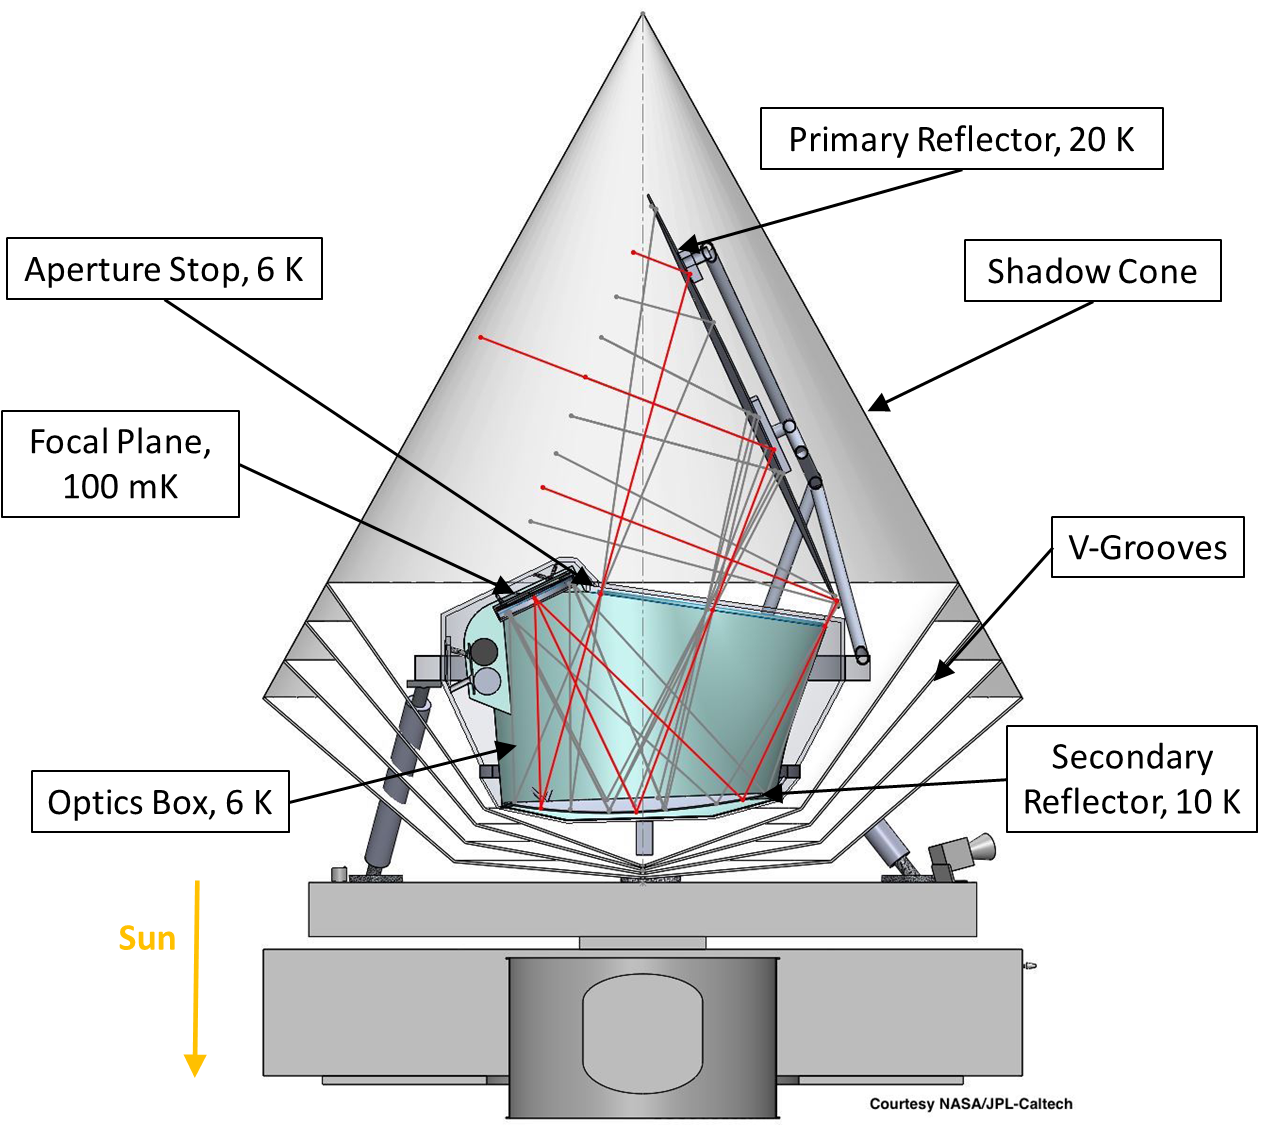
\includegraphics[height=9cm]{PICO_CAD_annotated.png}
%\end{tabular}
\end{center}
\caption { \label{fig:cad} 
Mechanical design of the PICO satellite. Components relevant to this paper are labeled, for other details see Sutin~et~al.\cite{brian_spie}
The symmetry axis of the satellite precesses around the satellite-sun axis (orange arrow) with an angle of 26 deg. This precession defines the 
shadow cone which is shown in light gray.
%\comb{%is the primary really at 15 K? hard to believe. Need to verify. 
%To explain the idea of a 'shadow cone', need to say something 
%about where the Sun is and how it illuminates the spacecraft such as to give this 'shadow cone'. }
%Primary 17 K, secondary 8 K, liner 6 (may get to 4.5 K)} 
}
\end{figure} 

% \begin{itemize}
% \item Sketch out satellite systems. Include CAD model figure and table of system parameters
% \subitem thermal systems and surface temperatures (NOTE! a bunch of these in Brian's paper don't match what we have used.  filters 1 K, stop 4.5-6 K, secondary 10 K, Primary 20 K, maybe others. Unclear how much of this will be in final version.
% \subitem sunshields and scan strategy
% \subitem observing frequency ranges 
% \item Summarize mission 
% \subitem L2 orbit, for earth-moon viewing angles
% \subitem 5 yrs active time frame
% \subitem launch vehicle is Falcon 9 
% \end{itemize}


\section{OPTICAL SYSTEM}
\label{sec:optics}

The PICO telescope is a 1.4~m aperture modified open-Dragone.  This choice was driven by a combination of science
requirements and the physical limits discussed in Section~\ref{sec:spacecraft}.  The science requirements are: a large diffraction 
limited field of view (DLFOV)\footnote{ We consider an area in the FOV diffraction limited when the Strehl ratio is 
larger than 0.8.} sufficient to support $\mathcal{O}(10^4)$ detectors, arcminute resolution at 800~GHz, low 
instrumental polarization, and low sidelobe response. Additionally, 
the transition edge sensor bolometers baselined for PICO require a telecentric focal plane which is sufficiently flat that it 
can be tiled by 10~cm detector wafers without reduction in optical quality. 

More than 30 years ago Dragone analyzed the 
performance of several off-axis systems and found solutions with low cross-polarization at the center of the field 
of view and with astigmatism, or astigmatism and coma, canceled to first order.\cite{dragone,dragone_coma,dragone1983} 
A number of recent CMB instruments used off-axis systems, and several 
began the design optimization with systems based on designs by
Dragone\cite{planck2000_optics,ACT2011_optics,SPT2008_optics,core2018_inst,LB2016_optics,parshley_ccat_spie}. 
For PICO we begin 
the optimization with a Dragone system that to our knowledge has not been implemented in CMB instruments before. 
We call it an `open-Dragone' because of its overall geometry and in contrast to the widely used `cross-Dragone', see Figure~\ref{fig:ray}. 

%\comr{I am confused about the previous paragraph. It starts with a claim of a quantitative 'comparison' between a number of 
%systems; it even presents the advantages of a particular figure of merit, but in the
%end it is largely a set of qualitative arguments.  Here is my version of this paragraph. }
%\como{I agree the rewritten strucutre is better.  I refined it some more.}

We consider two additional Dragone systems, a Gregorian Dragone and a cross-Dragone, and compare the 
relative performance of all three systems in terms of DLFOV, compactness, and rejection of sidelobes.  
Compared to the open-Dragone, the Gregorian has half the DLFOV for the same $F$-number and cannot  
support $\mathcal{O}(10^4)$ detectors. It is therefore rejected.  
The cross-Dragone has roughly $4\times$ the DLFOV of the open-Dragone, 
but is more difficult to pack inside the spacecraft volume while avoiding the known sidelobes shown in Figure~\ref{fig:sidelobes}.
We find the largest cross-Dragone which meets the PICO volume constraints has 
a 1.2~m aperture and an $F$-number of 2.5, while the largest open-Dragone aperture is 1.4~m with an $F$-number of 1.42. The larger 
$F$-number of the cross-Dragone system implies a larger physical focal plane, and therefore higher mass and cost, 
for the same number of pixels. 
%Although the 1.2~m cross-Dragone can accommodate a larger DLFOV, we could not mitigate
%its sidelobes without further reducing the aperture. 
For the PICO case, we conclude that the advantages of a low $F$-number and easily baffled sidelobes make the open-Dragone a good starting  
point for further optimization. 


%A cross-Dragone will always have a larger $F$-number 
%than an open-Dragone of the same aperture size, because the cross-Dragone focal length must be long enough that the focal plane 
%does not block the primary mirror. } 
% \comr{Can you really make such a general claim? }
%\comr{why does it 'always' have larger F? Can make a smaller F, no?}. \como{The smallest $F$-number of a crossed system is about 2. The focal length has to be long so the focal plane doesn't block the primary. You could make an open with F > 2, but you can't make a crossed system with F < 2.}

\begin{figure} [ht]
\begin{center}
%\begin{tabular}{c} %% tabular useful for creating an array of images 
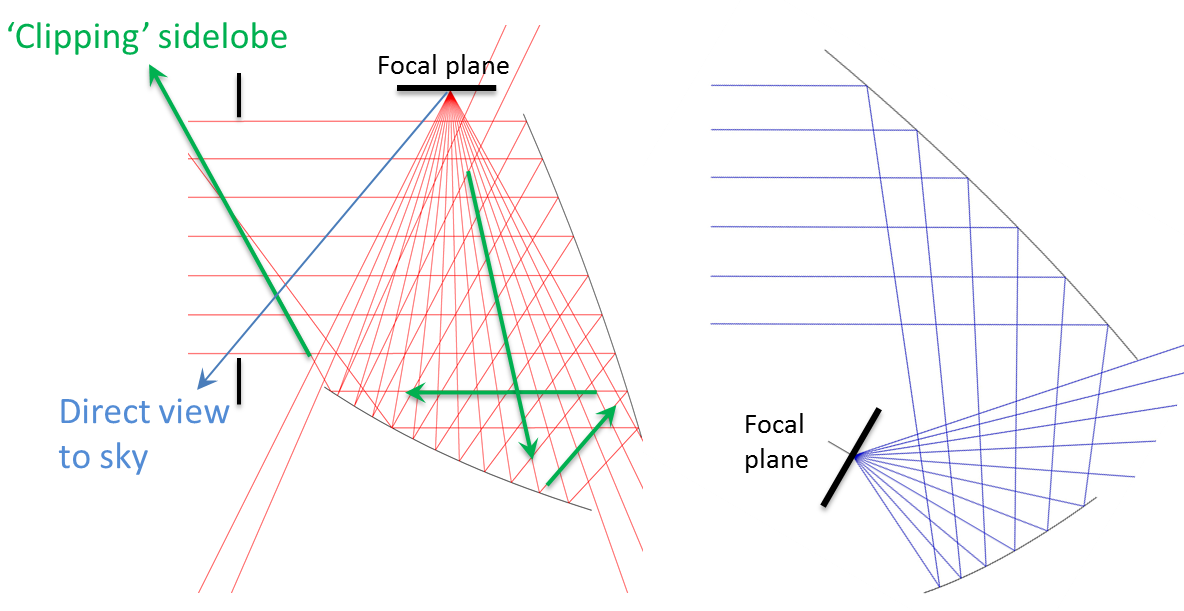
\includegraphics[height=6.5cm]{sidelobes.png}
%\end{tabular}
\end{center}
\caption { \label{fig:sidelobes} 
Comparison of sidelobes for a cross-Dragone (left) and an open-Dragone (right).  Rays are traced from the center 
of the focal plane toward the sky.
For both systems spillover around the secondary is straightforward to mitigate with absorptive baffles.  
However, the sidelobe and direct 
sky view in the cross-Dragone system require a long forebaffle or large $F$-number to mitigate, both of which are problematic in the PICO case.
}
\end{figure} 

We design the initial open Dragone following Granet's method\cite{granet2001}. 
We find a solution with low $F$-number, $F=1.42$, the largest aperture that satisfies the volume constraints, and a large 
DLFOV.  We force a circular aperture stop 
between the primary and secondary mirrors and numerically optimize its angle and position to obtain the best 
optical performance.  The stop diameter provides an effective 1.4~m aperture on the primary for the center feed.  
Adding a stop in this way increases the size of the primary mirror, because the primary is unevenly illuminated at various 
field angles.
Actively cooling the aperture stop, however, reduces detector noise, and the stop shields the 
focal plane from stray radiation. At this stage the system still meets 
the Dragone condition and is defined by the `Initial Open-Dragone' parameters in Table~\ref{tab:optics}.

In his publications Dragone provides a prescription to eliminate coma
in addition to the cancellation of astigmatism in the baseline designs.\cite{dragone_coma} The reflector corrections 
involve adding distortions to the primary and secondary reflectors 
which are proportional to $r^4$ where $r=0$ is at the chief ray impact point on each mirror. 
We thus attempt to increase the DLFOV using two methods. 

In the first method, one of the coauthors (RH) used Zemax to add Zernike 
polynomials to the base conics which describe the mirrors. These Zernike polynomials are offset from the symmetry axis of the conic 
by $624.2$~cm for the primary and $76.1$~cm for the secondary.  
This places the origin of polynomials at the chief ray impact point for each mirror. 
Inspired by the Dragone corrections, all Zernike terms up to fourth order and the first fifth order term are allowed to vary. 
The optimization metric is minimization of the rms spot diameter at 
the following locations: the center of the FOV, $\pm2$~deg in Y, and $\pm4$~deg in X. The center of the FOV is given a weight of 100
while each outer point is given a weight of 1. To constrain the optimization, the X and Y 
effective focal lengths are held fixed as is the impact point of the chief ray on the focal plane. 
This optimization step increases the DLFOV
by factors of 1.15, 2.4 and 10.5 at 21, 155 and 799~GHz, respectively. 
We improve the DLFOV at all frequencies by approximately 50\% by rerunning the optimization and including a curved focal surface. A small ($\sim$4\%) additional gain in DLFOV is achieved by adding Zernike terms 
up to sixth order, allowing the secondary to focal surface distance to vary, adding a weighted constraint on the effective focal length, 
and adding fields with weight of 0.01 to the rms spot diameter metric at $\pm7.5$~deg in Y and $+15$~deg in X. 
These additional fields are necessary to constrain the corrections at the mirror edges.

% \comr{The other method by Richard has the first step of converting the conics into an on axis XY polynomial representation. Then a similar procedure is followed.  It is less well behaved during optimization.  This second Richard method is what I replicated in CodeV.}
% \comb{is this 'other method' = method2? or is it 1b? \como{KY: My method is 1b and not discussed here.}}


\begin{figure} [ht]
\begin{center}
%\begin{tabular}{c} %% tabular useful for creating an array of images 
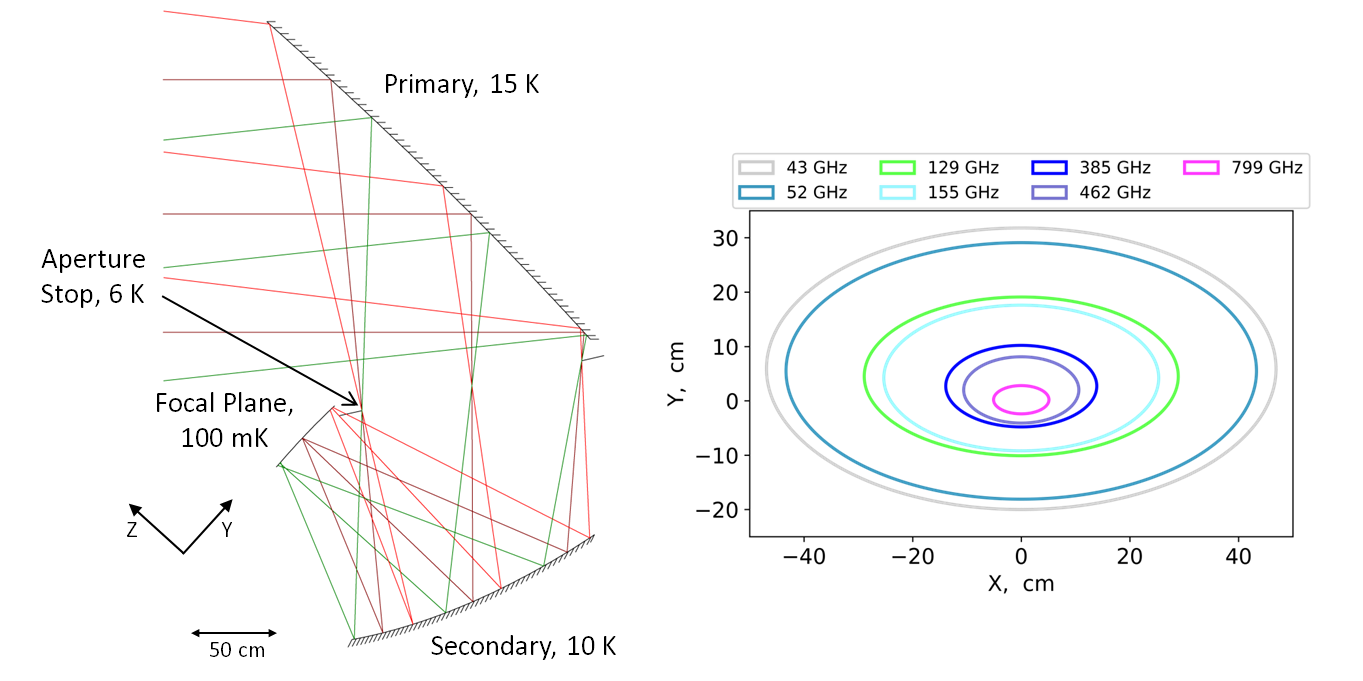
\includegraphics[height=7.5cm]{jpl_ray_strehl.png}
%\end{tabular}
\end{center}
\caption { \label{fig:ray} \label{fig:strehl} 
Raytrace (left) and Strehl~$=0.8$ contours (right) for the PICO optical design.
}
\end{figure} 

\begin{table}[ht]
\centering
\caption{Telescope geometric parameters  \label{tab:optics}}

\begin{adjustbox}{width=1.05\textwidth}
\hspace{-1cm}
\begin{tabular}{|l|llll||ll|}
\hline
\multicolumn{5}{|c||}{PICO optical system}                                    & \multicolumn{2}{c|}{Initial Open-Dragone$^b$}     \\ \hline
                          & Primary           & Secondary    & \multicolumn{2}{c||}{Telescope parameters$^b$} & \multicolumn{2}{c|}{Fundamental design parameters}  \\
Mirror size$^a$ (cm)      & $270 \times 205$ & $160 \times 158$ & Aperture (cm)           & 140      & Aperture (cm)                  & 140   \\
Radius of curvature (cm)  & $\infty$         & 136.6             & $F$-number             & 1.42     & $\theta_0$ (deg)           & 90    \\
Conic constant, $k$       & 0                 & -0.926            & h (cm)                    & 624.2    & $\theta_e$ (deg)           & 20    \\
Normalization radius (cm) & 524.8             & 194.1             & $\alpha$ (deg)            & 74.2     & $\theta_p$ (deg)           & 140   \\
4th Zernike Coefficient (cm)  & 2018.4            & -61.1             & $\beta$  (deg)            &  62.3    & L$_m$ (cm)                     & 240   \\
9th Zernike Coefficient (cm)  & -37.0             & 16.7              & L$_m$ (cm)                &   229.3  &                                &         \\
10th Zernike Coefficient (cm) & -2919.8           & -15.1             & L$_s$ (cm)                &   140.5  & \multicolumn{2}{c|}{Derived parameters} \\ 
11th Zernike Coefficient (cm) & -1292.7           & 22.3              &                           &          & $F$-number                     & 1.42  \\   
12th Zernike Coefficient (cm) & 120.6             & -3.8             &   \multicolumn{2}{c||}{Focal Surface}  & h (cm)                         & 624.2 \\   
13th Zernike Coefficient (cm) & -74.5             & 4.9               & Ellipse major axes (cm)   & 69 x 45  & $\alpha$ (deg)                 & 38.6  \\   
19th Zernike Coefficient (cm) & -75.8             & 3.4               & Ellipse major axes (deg)  & 19 x 13  & $\beta$  (deg)                 & 101.4 \\   
20th Zernike Coefficient (cm) & -398.9            & 6.3               & Radius of curvature (cm)  & 455      & L$_s$ (cm)                     & 122.2 \\   
21st Zernike Coefficient (cm) & -319.5            & 23.3              &                           &          & Primary, $f$ (cm)              & 312.1 \\   
22nd Zernike Coefficient (cm) & -276.6            & -8.5              &                           &          & Secondary, $a$ (cm)            & 131   \\   
23rd Zernike Coefficient (cm) & -201.6            & -3.2              &                           &          & Secondary, $e$                 &  1.802  \\
24th Zernike Coefficient (cm) & -127.4            & -1.9              &                           &          &                                &       \\
25th Zernike Coefficient (cm) & -55.0             & 0.1               &                           &          &                                &       \\\hline
\multicolumn{7}{l}{\footnotesize  $^a$ The maximum physical size of the mirrors.}\\
\multicolumn{7}{l}{\footnotesize  $^b$ Telescope parameters follow the definitions in Granet 2001.\cite{granet2001}} \\
\end{tabular}
\end{adjustbox}
\end{table}

%To increase the optical performance we use CodeV to numerically optimize the system.  
In the second optimization method, another coauthor (JM) uses CodeV and allows more of the geometric 
parameters of the system to vary.  To adjust the 
mirror shapes, we add Zernike polynomial corrections to the conic surfaces which define the two mirrors.
The Zernike polynomials are defined on the same coordinates as the base conics.  
We vary the 4th and 9th-13th terms of the Zernike polynomials. We allow the focal surface curvature 
and focal surface to secondary distance L$_s$ to vary.  The primary-secondary distance L$_m$, primary offset $h$, 
and the primary and secondary rotation angles, $\alpha$ and $\beta$, are varied as well.  The optimization 
metric is the rms spot diameter across the field of view, with weighted constraints requiring telecentricity and 
maintaining the X- and Y-focal lengths.  We add Lagrange constraints 
to enforce beam clearances and place an upper limit on overall system size.  Once the optimization converges to 
an acceptable optical system, we add higher order Zernike terms, 19th-25th, and refine 
the mirror shapes using the same metric and constraints. 
The current PICO optical design is from this optimization procedure.

Figure~\ref{fig:compare} shows that the second optimization method greatly increases the DLFOV relative to the initial open-Dragone design.  
The DLFOV is increased by factors of 1.9, 3.8, 4.3, and 4.6 at 21, 129, 155, and 799~GHz, respectively.  
The most important gain is at 129 and 155~GHz where the extra area allows us to add 
many more `C' and `D' pixels, see Figure~\ref{fig:bands} and Section~\ref{sec:focalplane}, 
which contain the bands most sensitive to the CMB. 
Being able to pack 100's of `C' and `D' pixels into the focal plane is what allows PICO to reach unprecedented levels of CMB sensitivity. 
Compared to the first optimization method, the second gives somewhat better performance at the lower frequencies, with 1.11 and 1.15 times large DLFOV at 21 and 155~GHz, respectively.
Method two gives a smaller DLFOV at 799~GHz, only 0.3 times the method one area, but the DLFOV is still sufficient for the number of 799~GHz detectors we require. Figure~\ref{fig:compare} also shows the second optimization method reduces the overall telescope volume, allowing it to fit more easily within the shadow cone. 

\comr{do you mean if we had only optimization method 1 we wouldn't reach our goals?} \como{not really, because the goals are poorly defined.  But total CMB sensitivity would be lower with method 1 only.}

The geometric parameters of the PICO optical system are given in Table~\ref{tab:optics}. The 
system is diffraction limited for 799~GHz at the center of the field of view. At 155~GHz the 
DLFOV is 82.4~deg$^2$ and the total throughput for all frequencies is 910 cm$^2$sr. 
Figure~\ref{fig:strehl} shows Strehl of 0.8 contours for all pixel types.
The slightly concave focal surface, which has a radius of curvature of 4.55~m, is telecentric to 
within 0.12~deg across the entire FOV.

\begin{figure} [ht]
\begin{center}
%\begin{tabular}{c} %% tabular useful for creating an array of images 
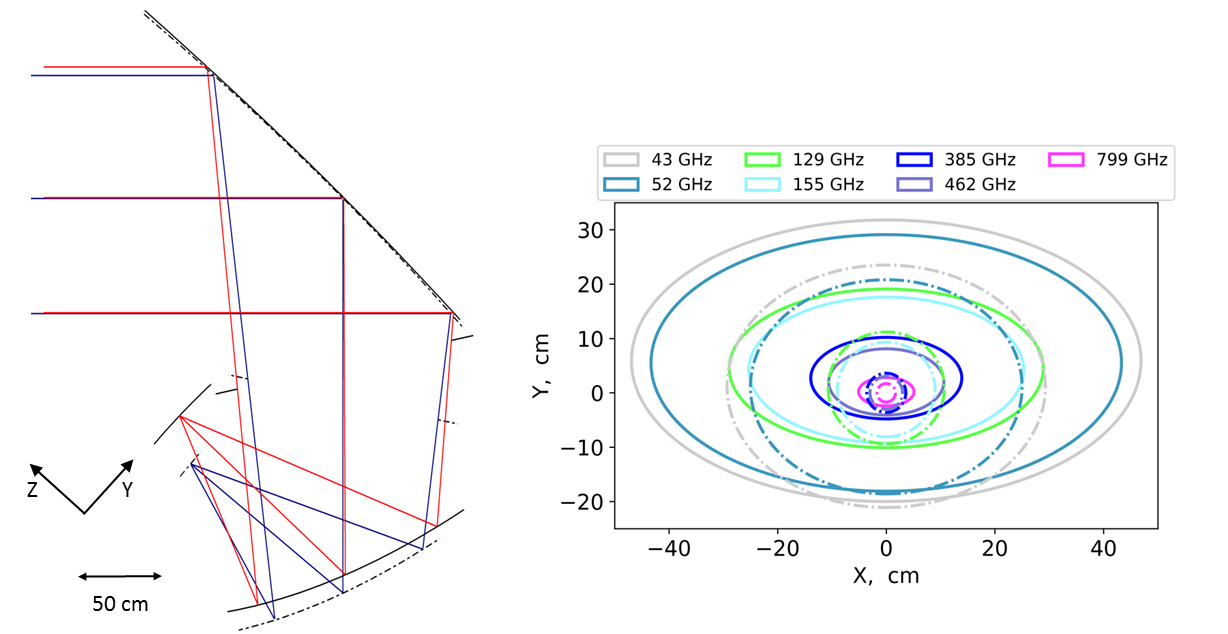
\includegraphics[height=7cm]{jpl_vs_V3D.png}
%\end{tabular}
\end{center}
\caption { \label{fig:compare} 
Comparison between the open-Dragone optimized using method two and the initial open-Dragone.  
The ray traces (left) are aligned at the chief ray impact point on the primary. 
The optimized system (red rays, solid mirrors) is smaller in the vertical direction than the unoptimized version 
(blue rays, dash-dot mirrors). The overlaid Strehl~$=0.8$ contours (right) show the improvement at 
all frequencies in the optimized (solid lines) system over the unoptimized (dash-dot lines) system. 
}
\end{figure} 

An additional benefit of the optimization is the concave focal surface. The open-Dragone's focal surface is naturally curved.  Matching this 
curvature reduces defocus and increases the DLFOV as well as increasing telecentricity.  The unoptimized system is telecentric to within 
2.5~deg while the optimized version is telecentric to within 0.12~deg. If the focal surface is too strongly curved tiling it with flat detector 
wafers would result in large defocus at the edges of these wafers.  This is not the case for PICO. The focal surface radius of curvature, 4.55~m, 
results in a defocus of 0.1~mm for the edge of a 10~cm wafer. 



\section{FOCAL PLANE}
\label{sec:focalplane}

Modern mm/sub-mm detectors are photon noise limited, therefore the primary way to increase sensitivity is to increase the 
number of detectors. 
\comr{are there additional secondary ways?}  % longer integration. higher throughput detectors (bandwidth). higher system effeciency (100% of bolo throughput reaches sky).  Could read 'major', 'most effective', or similar.  But not 'only'.
The PICO focal plane has 12,996 detectors, 175 times the number flown on \textit{Planck}. PICO achieves this by 
having a large DLFOV and using multichroic pixels (MCPs)\cite{Suzuki2014_samps,datta2014_mcp}. 
The MCP architecture assumed for PICO has three bands per pixel with two single polarization transition 
edge sensor (TES) bolometers per band and therefore six bolometers per pixel. 
We assume the MCPs are coupled to free space using lenslets and sinuous antennae \cite{Suzuki2014_samps}, 
but the focal plane layout, including pixel sizes, numbers, and spacing would not change significantly 
if horn or phased array coupling was used instead.

PICO has 21 overlapping bands with centers spanning the range 21--799~GHz. The bands are divided amongst 
nine pixel types labeled A to I; see Figure~\ref{fig:bands}. 
%These bands provide the broad fequency coverage needed to seperate the CMB, Galactic dust, and various foregrounds using their differing spectra.  \comr{no. it is needed to achieve all of our science goals. separating foreground is only one of the goals of the broad frequency coverage.}
The 25\% fractional bandwidth is broader than the interband spacing causing neighboring bands to 
overlap and requiring them to be in separate pixels. 
%For example, bands 1, 3, and 5 are in pixel A while bands 2, 4, and 6 are in pixel B.  This 
%complicates the pixel design and focal plane layout, but allows broader bands which increases total sensitivity.  
%\comb{Be more succinct. A paper is not a tutorial. I don't agree that it leads to more complications}
The exceptions to the MCP architecture are the highest three bands, because they are above the superconducting 
band gap of niobium which is used for the transmission lines, antennae, and filters of the MCPs.  
For bands G, H, and I, we will use feedhorn-coupled polarization sensitive bolometers. The technology has high TRL 
as it has already been used successfully with 
\textit{Planck}\cite{planck2010_hfi} and Herschel SPIRE\cite{spire2010}.

\begin{figure} [ht]
\begin{center}
%\begin{tabular}{c} %% tabular useful for creating an array of images 
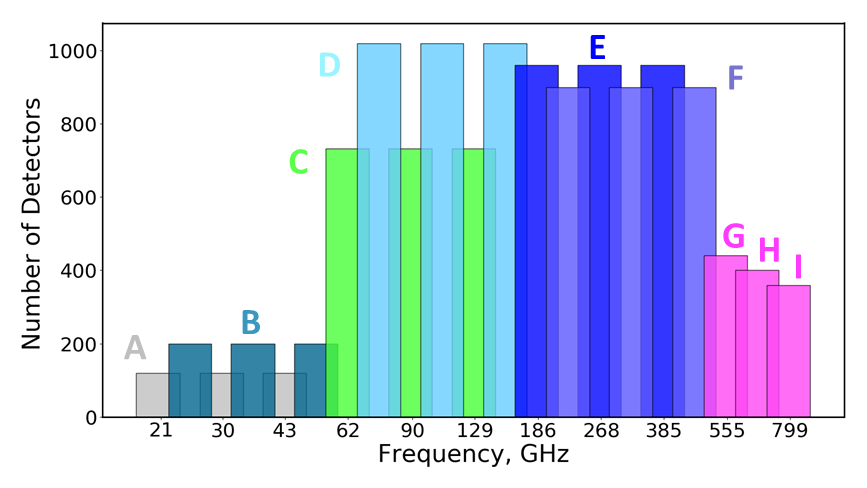
\includegraphics[height=6cm]{bands_label.png}
%\end{tabular}
\end{center}
\caption { \label{fig:bands} 
Frequency coverage of the PICO bands. Each color (excluding magenta) denotes a different MCP, labeled A-F. The bar height 
indicates the number of detectors per band.  Bar width gives the bandwidth. All bands are top-hats with 
25\% fractional bandwidth; the $x$-axis is logarithmic.  The three highest frequencies (magenta) are the 
single color pixels G, H, and I.}
\end{figure} 

Figure~\ref{fig:focal_plane} shows the PICO focal plane.  
We optimize the diameter of each MCP by calculating the array sensitivity for that pixel type. The calculation includes the 
increased illumination of the aperture stop as the pixel diameter decreases, as described in Section~\ref{sec:det_noise}.
We choose a pixel diameter of $2.1$F$\lambda_{\rm mid}$, where $\lambda_{\rm mid}$ refers to the center 
band of each pixel. This gives an edge taper, $T_e$, on the stop of 10~dB for the center band of each pixel. 

%We hex-pack pixels onto 94~mm hexagonal wafers to minimize wasted space for the mid-frequency pixels. 
%The three central wafers have the same 94~mm hexagon footprint but are split into 
%3 rhombi, shown in Figure~\ref{fig:focal_plane}, because the highest frequency magenta wafer will use different 
%detector technology and will need to be fabricated separately.  \comb{I don't understand the last few sentences. Need to discuss}
%The 3 central wafers are rhombi to put the F pixels on different wafers than the G, H, and I pixels, which use different technology. The C and D/E wafers are 94~mm regular hexagons. 


% The PICO focal plane is designed to take maximum advantage of the large field of view.  The optical quality peaks at the 
% focal plane center and falls off with radius as shown in Figure~\ref{fig:strehl}.  This pattern dictates the layout shown 
% in Figure~\ref{fig:focal_plane}. The highest frequency pixels are centered on the focal plane and low frequency pixels are arranged 
% around the edge. The maximum radial distance for a given pixel is the point where 
% the Strehl ratio for the upper edge of the highest frequency band within that pixel equals 0.8.  Interior to these contours, the ellipses in 
% Figure~\ref{fig:focal_plane}, the Strehl ratio increases ensuring pixels are diffraction limited.
% \comb{most of the text in this paragraph is relatively trivial (including the first sentence). Can prune and make more succinct.}


\begin{figure} [ht]
\begin{center}
%\begin{tabular}{c} %% tabular useful for creating an array of images 
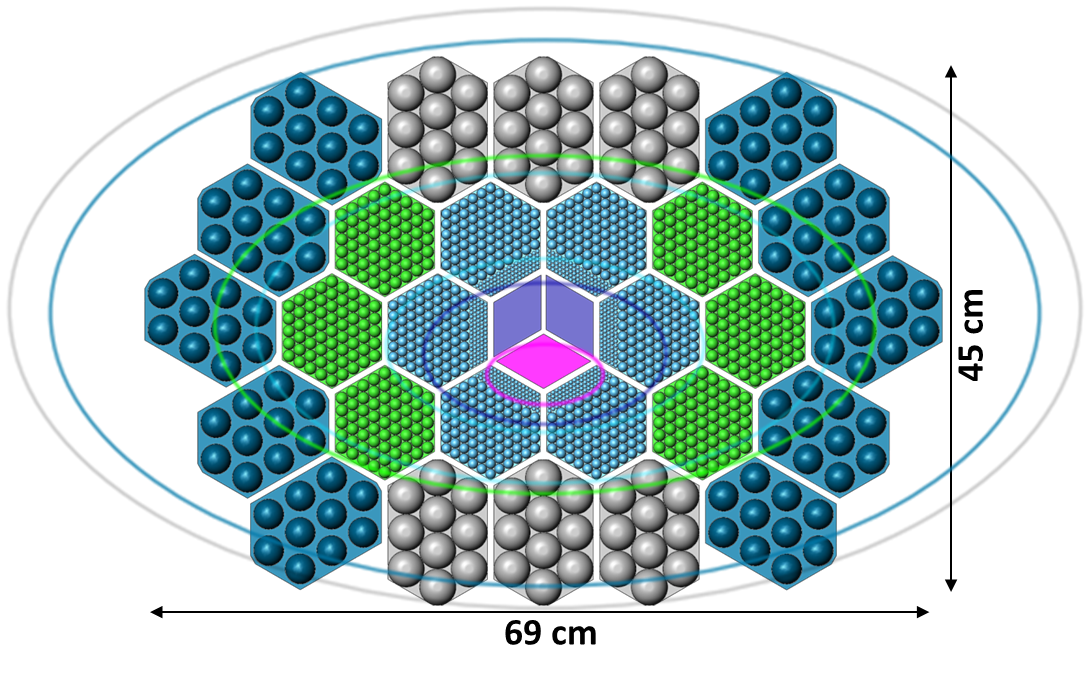
\includegraphics[height=7.5cm]{version3_focal_plane.png}
%\end{tabular}
\end{center}
\caption { \label{fig:focal_plane} 
PICO focal plane layout with Strehl~$=0.8$ contours for each pixel type. The pixel and Strehl contour colors match the band colors, A-I, 
in Figure~\ref{fig:bands} }
\end{figure} 


% \sout{Optimizing the pixel size is a balance between the total number of pixels, $N_{px}$, and the efficiency with which 
% they couple to the telescope. Smaller pixels pack more densely on the focal plane, $N_{px}\propto 1/D_{px}^2$, but over 
% illuminate the stop which reduces optical efficiency and adds optical load.}  \comb{instead of making general statements
% that have a tutorial flavor, just say what you do}

% \comb{We optimize the pixels diameters for each MCP by calculating the mapping speed. The calculation includes the 
% increased illumination of the aperture stop as the pixel size decreases, as described in more detail in Section ... }
% %Since PICO has a cold stop additional load is minimized, reducing the penalty for smaller pixels.  
% We choose a pixel diameter of $2.1$F$\lambda_{mid}$, where $\lambda_{mid}$ refers to the center 
% band of each pixel. This gives an edge taper, $T_e$, on the stop of 10~dB for the center band. 
% \sout{Due to the multichroic nature of the pixels $T_e$ varies with band, details in Section~\ref{sec:noise}}. 
% We hex-pack pixels onto 94~mm hexagonal wafers to minimize wasted space for the mid-frequency pixels. 
% The three central wafers have the same 94~mm hexagon footprint but are split into 
% 3 rhombi, shown in Figure~\ref{fig:focal_plane}, because the highest frequency magenta wafer will use different 
% detector technology and will need to be fabricated separately.  \comb{I don't understand the last few sentences. Need to discuss}

% order 0.5 sec is longer than the sample time even at 1 deg beams. sweeping 1 deg takes 0.2 sec.
%\sout{The polarization sensitive bolometers in each MCP are oriented perpendicular to each other. }
Differencing detectors that are sensitive to orthogonal polarization states enables each pixel to make a measurement of 
a particular Stokes parameter. Pixels that are sensitive to the $U$ Stokes parameter are rotated by 45~deg relative to those
that are sensitive to $Q$. This Q/U measurement is in the instrument reference frame with the $x$-axis parallel to the scan 
direction; see Figure~\ref{fig:QU}. 
%\sout{ This layout reduces systematic errors by maximizing the number of Q,U pixel pairs which have almost identical optical paths and measure sky locations as close to simultaneously as possible.  }

\begin{figure} [ht]
\begin{center}
%\begin{tabular}{c} %% tabular useful for creating an array of images 
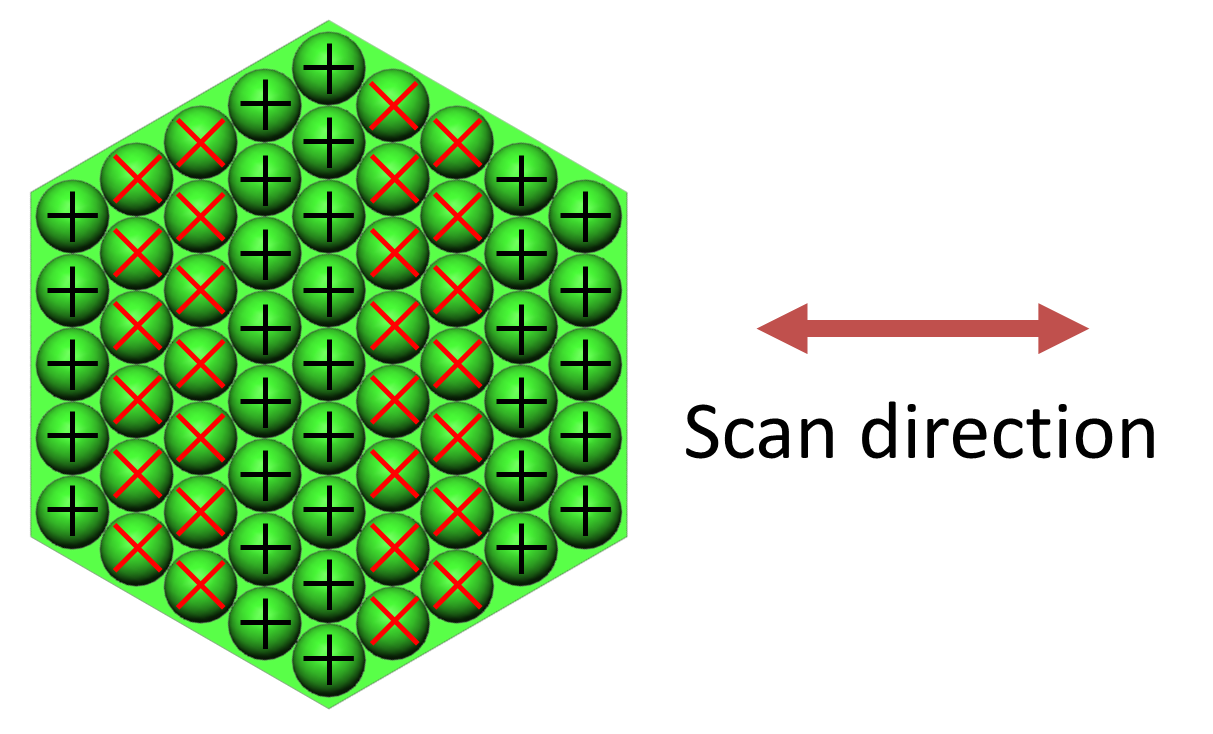
\includegraphics[height=4cm]{QU_wafer.png}
%\end{tabular}
\end{center}
\caption { \label{fig:QU} 
Layout of pixels sensitive to Stokes Q (black crosses) and Stokes U (red exes) for an example wafer.}
\end{figure}

%\sout{Two multiplexing methods, time domain (TDM) and frequency domain (FDM), were explored for PICO. Trade-off details are discussed in Sutin et~al.\cite{brian_spie}}
The PICO focal plane readout has been designed around $\times$128 time domain multiplexing (TDM), but this choice is not a 
significant driver for the focal plane layout or overall noise budget. 


\section{INSTRUMENT NOISE}
\label{sec:noise}
%\comr{comment somewhere in this section that these noise numbers are CBE. no margins.}

We develop an end to end noise model of the PICO instrument to predict full mission sensitivity and 
provide a metric by which to evaluate mission design trade-offs.  This model assumes white noise
at all frequencies. 
%\comr{to the extent you can, state what you do, rather than what you don't do}. 
The overall sensitivity does not include calibration uncertainties or estimates of other possible 
systematic effects. 
%\comr{but this is an example in which we state what we don't include...} 
To construct the model we estimate the 
optical load, calculate noise equivalent power (NEP) by source, 
combine all NEP terms to get detector noise, combine all detectors to get noise per frequency band, and then 
include total mission time to find overall mission sensitivity.\cite{suzuki2013_thesis,aubin2013_thesis}  
Each of these steps includes various assumptions and design decisions, 
which are discussed in this section.  The assumptions are summarized in Table~\ref{tab:assume}.

\comr{what's important here is how do we know that the model is correct. How was it checked and validated?} \como{See following.  An aside, what is the normal or natural way to 
refer to work done by coauthors on the paper?  Saying 'we' all the time seems odd, but so does talking about work done by coauthors as if it is seperate from the 
main work written up in this paper.}\\
To validate our model we compare to an independent calculation done by collaborators at JPL.  The calculations agree within 1\% for individual noise terms 
and for overall mission noise.  We also use our model to calculate CORE and LiteBIRD noise using published system parameters. The 
results are consitent with published values.  Additionally, we compare PICO detector noise to CORE and LiteBIRD detector noise.  The 
lower PICO noise is explained by the cold system and differing optical efficiency.  From these test we conclude that our model is correct and our assumptions 
are reasonable.
\como{I'm not a huge fan of this paragraph.  It is fairly wishy-washy, but is the best I can do for now.}


\begin{table}[ht]
\centering
\caption{Noise model parameters, see text for details. }
\label{tab:assume}
%
\begin{tabular}{|l|l|}
\hline
%                                 &                                                  \\
Throughput                       & single moded, $\lambda^2$          \\
Fractional Bandwidth             & 25\%                                             \\
Mirror emissivity                & $\epsilon = \epsilon_0\sqrt{\nu/\text{150~GHz}}, \epsilon_0 = 0.07\%$ \\
Aperture stop emissivity         & 1                                                \\
Low pass filter reflection loss  & 8\%                                                \\
Low pass filter absorption loss$^a$  & frequency dependent, 0.2\%--2.8\%             \\
Bolometer absorption efficiency  & 70\%                                             \\
T$_e$ of low, middle, and high bands (dB) & 4.8, 10.0, 20.7                                               \\
$\eta_{\rm stop}$ of low, middle, and high bands & 0.68, 0.90, 0.99   \\
Bose noise fraction, $\xi$       & 1                                                \\
Bolometer yield                 & 90\%                                             \\
Bath temperature, $T_o$ (mK)    & 100                                              \\
TES critical temperature, $T_c$ (mK)   & 187                                              \\
Safety factor, P$_{\rm sat}$/P$_{\rm abs}$      & 2                                                \\
Thermal power law index, $n$    & 2                                                \\
Intrinsic SQUID noise (aW/$\sqrt{\text{Hz}}$)   & 3                        \\
TES operating resistance, $\Omega$    &  0.03                               \\
TES transition slope, $\alpha$    & 100                                         \\
TES loop gain                    & 14                                \\
Mission length (years)           & 5                                                \\
Observing efficiency             & 95\%                                             \\
%Multiplexing factor              &
%Number of rows/columns/whichever matters . .. 
%\comr{other?}                    &                                                  \\
\hline
\multicolumn{2}{l}{\footnotesize $^a$Assumes seperate metal mesh in polypropylene filters for each wafer.}
\end{tabular}
\end{table}


\subsection{Single bolometer noise}
\label{sec:det_noise}

\subsubsection{Model}

The sources of optical load are the CMB, the primary and secondary mirrors, the aperture stop, and a low pass optical filter.  
These elements are shown schematically in Figure~\ref{fig:load}. 
The total load absorbed at the bolometer is the sum of the power emitted by each element reduced by the transmission 
efficiency of the elements between the emitting surface and the bolometer.  
The absorbed power is
\begin{equation}
\label{eq:load}
P_{\rm abs} =  (((( P_{\rm CMB} \eta_{\rm PRI} + P_{\rm PRI} ) \eta_{\rm stop} + P_{\rm stop}(1-\eta_{\rm stop}) ) \eta_{\rm SEC} + P_{\rm SEC})\eta_{\rm filter} + P_{\rm filter}) \eta_{\rm bolo},
\end{equation} 
where $P_{\rm elem}$ is the in band power emitted by a given element for a single polarization and $\eta_{\rm elem}$ is the 
transmission efficiency 
of the element. Power emitted by the stop is a special case. We multiply $P_{\rm stop}$ by 
$(1-\eta_{\rm stop})$ because $\eta_{\rm stop}$ is the spillover efficiency, the fraction of the throughput which passes through the 
stop. Therefore $(1-\eta_{\rm stop})$ is the fraction of the throughput which views the stop. 


\begin{figure} [ht]
\begin{center}
%\begin{tabular}{c} %% tabular useful for creating an array of images 
\hspace{1cm} 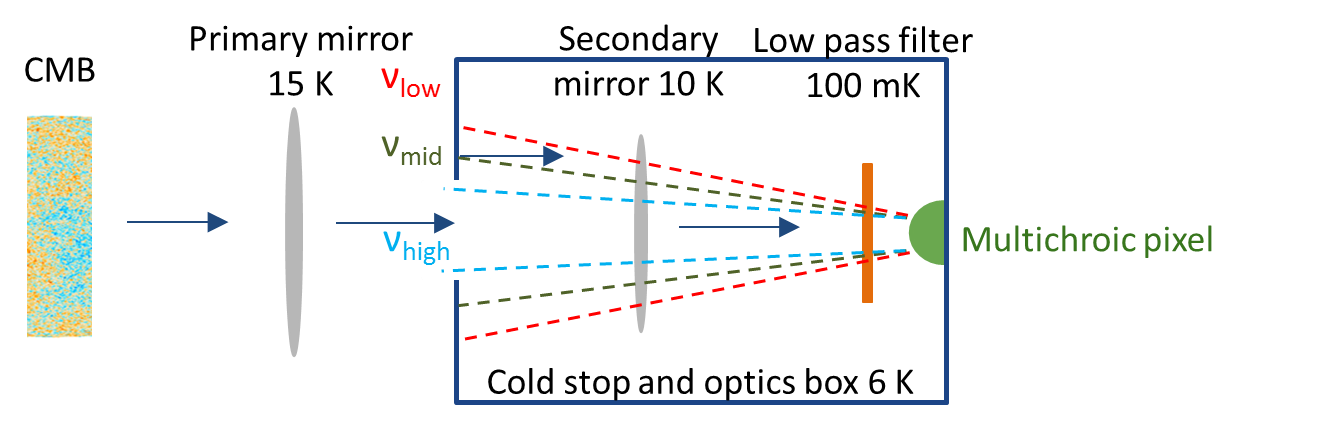
\includegraphics[height=5cm]{load_calc_MCP.png}
%\end{tabular}
\end{center}
\caption[load] { \label{fig:load} 
Schematic representation of the prediction of optical load.  Power emitted by each element is modified by the efficiency of 
the following elements and added to the total expected load.  The multichroic pixel illuminates the stop differently for 
each of the three bands. }
\end{figure} 
%

%For PICO, the CMB and stop dominate the optical loading up to 400~GHz, as illustrated by the shape of the optical load 
%curve in Figure~\ref{fig:popt} which roughly follows a 4--6 kelvin blackbody.  Even at 800~GHz the CMB and stop are the 
%largest optical load, accounting for 12\% more power than the mirrors. 
%\comr{how do I see this from the figure? Is that true at all frequencies?}
For PICO, the CMB and stop account for the majority of the optical load at all frequencies. 
The jumps in load between neighboring bands, seen in Figure~\ref{fig:popt} around 70 and 200~GHz, are 
due to $\eta_{\rm stop}$ changing with frequency which is a consequence of using MCPs.  
The MCP angular beam width depends on the wavelength and pixel diameter as\cite{suzuki2013_thesis}
\begin{equation}
\label{eq:mcp_beam}
\theta_{1/e^2} = \frac{2.95 \lambda}{\pi D_{\rm px}}. 
\end{equation} 
The edge taper, T$_e$, of the middle frequency band in each pixel is chosen to be 10~dB. For the upper and lower bands 
T$_e$ is calculated using Equation~\ref{eq:mcp_beam}. This changing illumination of the stop is shown schematically by 
the dashed rays in Figure~\ref{fig:load}. 
For each MCP in pixels A-H T$_e$ is 4.8, 10, and 20.7~dB for the lower, middle, and upper bands, respectively.  These 
edge tapers correspond to $\eta_{\rm stop}$ of 0.68, 0.90, and 0.99.
The changing $\eta_{\rm stop}$ has two main effects; changing optical efficiency between bands, which affects optical load 
and the NEP to noise equivalent temperature (NET) conversion, and telescope beam size not scaling smoothly with $\lambda$.

\begin{figure} [ht]
\begin{center}
\begin{tabular}{ccc} %% tabular useful for creating an array of images 
%\includegraphics[height=8cm]{P_optical.png}
\hspace{-1.4cm} 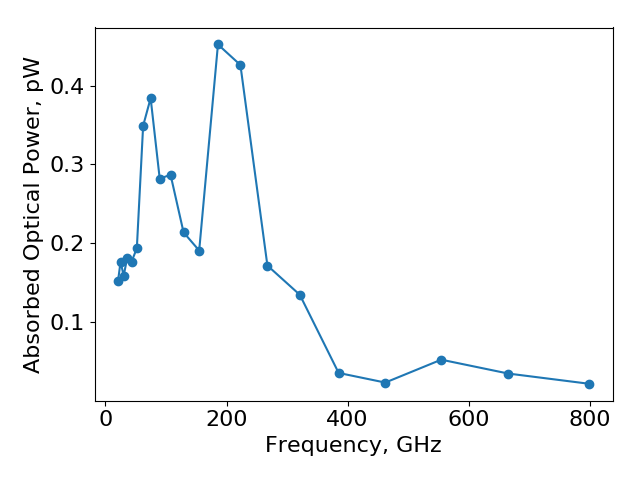
\includegraphics[height=4.9cm]{system_Popt.png} & \hspace{-0.7cm} 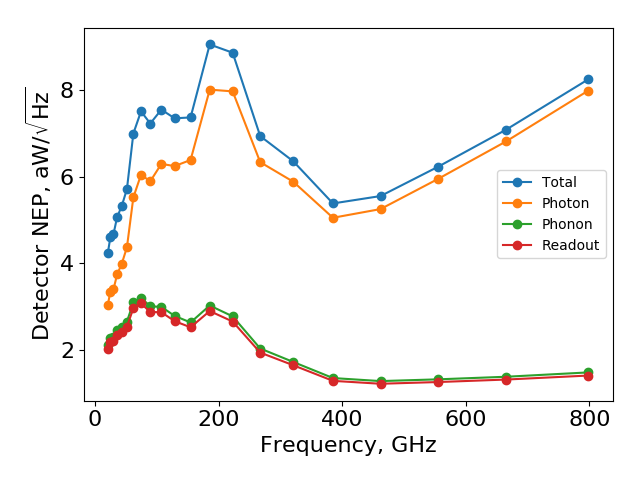
\includegraphics[height=4.9cm]{system_NEP.png} &\hspace{-0.7cm}  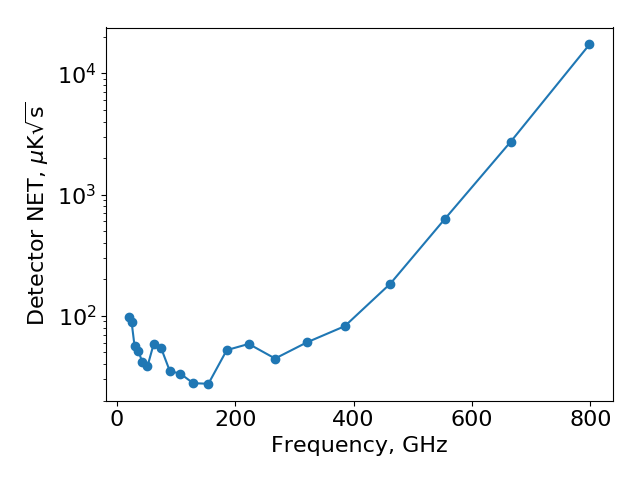
\includegraphics[height=4.9cm]{system_NET.png} 
\end{tabular}
\end{center}
\caption{ \label{fig:popt} \label{fig:noise} \label{fig:net} 
Left: Expected optical load as a function of frequency for single polarization PICO bolometers. 
Center: Breakdown of NEP across the PICO frequency range.  Photon noise dominates even at the lowest frequencies. 
Right: Single detector NET, temperature sensitivity \comr{what does that mean?} \como{as opposed to polarization sensitivity which is lower by $\sqrt{2}$.
Although maybe that is obvious as it is for 1 detector?}, across the PICO bands. 
}
\end{figure} 

We consider four noise sources per bolometer; photon, phonon, TES Johnson, and readout. 
Photon noise depends on the absorbed power\cite{richards1994}, 
\begin{equation}
\label{eq:photon}
NEP_{\gamma}^2 = \int\limits_{\rm band} 2h\nu p_{\nu} \, d\nu + 2\xi \int\limits_{\rm band} p_{\nu}^2 \,  d\nu,
\end{equation} 
where $p_{\nu}$ is the power spectral density for a single polarization absorbed at the bolometer and $\xi=1$ is the fraction of correlated Bose 
photon noise. We include a factor of 2 in the Bose noise term because the bolometers receive the power from a single 
polarization. 
From $P_{\rm abs}$ we calculate the TES bolometer properties and phonon noise.\cite{mather1982}  
The last noise term intrinsic to the bolometer is the TES Johnson noise \comr{aren't we using the same
Johnson noise for all bolos?} \como{I don't understand this question.  All bolos have Johnson noise, but it depends on voltage bias, so it varies band to band.}. All noise sources in the cold and warm readout 
electronics are lumped under the readout term.  The NEPs for each noise source as a function 
of frequency are shown in Figure~\ref{fig:noise}.


\subsubsection{Results}  % not the best word to distinguish these two subsubsections.

The primary driver of noise levels is the optical load.  The combination of the CMB and aperture stop make up the 
majority of the load in all bands. The load from the mirrors is greatest at 799~GHz where it is 47\% of the total 
optical load. The CMB provides more than half the load 
in the middle and upper bands of the multichroic pixels, but the stop dominates the load in the lowest band of each pixel.  
Load from the stop in the lowest band of each pixel ranges from 1.2 times the CMB load at 21~GHz to a maximum of 4.7 
times the CMB load at 223~GHz. 

For PICO, photon noise dominates at all frequencies as shown in Figure~\ref{fig:noise}. Bose noise is most significant 
at lower frequencies with NEP$_{\rm Bose}$/NEP$_{\rm Poisson}= 1.5 $ in the lowest band.  However, Poisson noise increases as 
$\sqrt{P_{\rm abs}\nu}$ while Bose is proportional to $P_{\rm abs}$, so Poisson noise equals Bose noise at 30~GHz and dominates at higher bands; 
%\comr{the scaling of the ratio is important, not just the scaling of the Poisson term}
NEP$_{\rm Bose}$/NEP$_{\rm Poisson} <10\%$ at 321~GHz. 
Phonon noise is the second most significant source, NEP$_{\rm phonon}$/NEP$_{\rm photon}$ ranges from 65\% at 21~GHz 
to 19\% at 799~GHz. 
% this is NEP/NEP NOT squared.  Squared is 2.2 at 21 GHz and 0.01 at 321. < 10 at 129 GHz.  in NEP to NEP bose = poisson at 30 GHz


For TDM readout, phonon and readout noise are roughly equal with TES Johnson noise being insignificant.  We also modeled 
frequency domain multiplexing (FDM) readout.  For FDM the TES Johnson noise is higher, 2/3 of the readout NEP, but the readout 
noise is lower.  Comparing the combined TES Johnson and readout NEPs for TDM and FDM we find essentially indentical performance 
with total noise differing by less than 3\% across all bands.  For both systems we require a focal plane temperature, $T_o$, of 
100~mK and a bolometer safety factor of 2 to remain photon noise dominated at the lowest bands. 
\comr{should we have Dobbs review this?} \como{I don't think it is necessary. But you're more familiar with the politics of this one. Dobbs isn't a co-author, if that matters.}


% RESULTS 
% Readout noise depends on the assumption of FDM or TDM readout and includes all remaining noise sources, the Johnson noise of the TES as well as 
% all components not intrinsic to the bolometers.  
% For both multiplexing schemes NEP$_{readout}$ is dominated by the SQUID amplifier with moderate contributions from various resistors 
% and amplifiers in the readout chain. We calculate noise for both FDM and TDM systems, though TDM is the current baseline, and find both to 
% be below both photon and phonon 
% noise for all bands.  Both systems give similar noise levels, with total noise differing by less than 3\% in all bands.
%  which is below the fidelity of the current study. 
% Some thought has been put into optimizing the readout systems for space, but since the expected noise is already sufficiently low this was not pursued 
% in detail. 
% For TDM and FDM the noise primarily scales with TES bias voltage which depends on the electrical power needed to operate the TES, 

%discussion of primary scalings and drivers? Popt does it all. choices like 100 mK and P/P = 2.
% The noise breakdown in Figure~\ref{fig:noise} drives various aspects of the PICO design. Since photon noise dominates at all frequencies and 
% photon noise scales with $\sqrt{P_{abs}}$, Equation~\ref{eq:photon}, the primary driver of noise is optical load.   The second largest source 
% of noise is phonon noise.  Combining
% Equations~\ref{eq:G} and~\ref{eq:phonon} we see $NEP_{phonon}$ scales with $\sqrt{T_C}$ and $\sqrt{P_{sat}}$.  Cooling the focal plane to 100~mK 
% reduces $T_c$ since $T_c \propto T_o$.  The saturation power depends on the choice of safety factor, $P_{sat}/P_{abs}$, as well as on optical load.  
% We choose safety factor of two to lower noise, while providing margin for unexpected loads or variations in $G$ of the fabricated 
% bolometers. Readout noise scales with $\sqrt{P_{sat} - P_{abs}}$, Equation~\ref{eq:readout}, which is reduced by reducing the safety factor or $P_{abs}$.  
% From this analysis we see that all noise sources depend on $P_{abs}$, either directly or through how load drives bolometer properties.  
% Therefore the 
% most straightforward way to reduce noise is to limit all optical loads other than the CMB.  This motivates the simple, few element telescope we 
% have designed with the aperture stop and secondary mirror actively cooled to reduce excess load and photon noise. 

\subsection{Combined  array noise}

Using single detector NEPs from Section~\ref{sec:det_noise} and the detector counts from Section~\ref{sec:focalplane} we 
calculate the combined NEP of the detector array for each band.  Combining detectors simply reduces noise by $\sqrt{N}$ 
except for Bose photon noise. For the lowest band of each MCP the pixels over sample the PSF, pixel spacing is $0.4$F$\lambda$, resulting in correlated 
Bose noise between pixels.  Accounting for this effect gives a 26\% increase in the combined array $NEP$ of the lowest band, 21~GHz, and  
a 0.003\% increase in array $NEP$ at the highest band, 799~GHz.  

From the array $NEP$ we convert to $NET$ per band,
\begin{equation}
\label{eq:NET}
\frac{NEP}{NET} = \sqrt{2} \, \eta_{\rm opt} \int\limits_{\rm band}\frac{dp_{\nu}}{dT}\Bigr|_{T_{\rm CMB}} d\nu.
\end{equation} 
The $\eta_{\rm opt}$ term contributes to the `jumps' in $NET$ seen in Figure~\ref{fig:net}, because $\eta_{\rm opt}$ varies band to band.  
%We use CMB temperature units for all bands, even though this isn't particularly suitable for the highest bands, because the CMB is the most stringent requirement on sensitivity.

All the above calculations are for sensitivity to temperature and are given in Table~\ref{tab:noise}.  Assuming evenly weighted observations 
of the full sky and 5 years observing at 95\% efficiency, we calculate full mission map sensitivities in polarization; final column in Table~\ref{tab:noise}.
Combining all bands gives a total CMB map depth for the entire PICO mission of 0.62~$\mu$K$_{\rm CMB}$-arcmin.

\begin{table}[ht]
\centering
\caption{PICO frequency channels and noise. }
\label{tab:noise}
\begin{tabular}{|c|c|c|c|c|c|c|cc|}
\hline
Pixel  & Band  & FWHM   & Bolometer NEP & Bolometer NET        & N$_{\rm bolo}$ & Array NET            & \multicolumn{2}{|c|}{Polarization map depth}  \\
Type   & GHz   & arcmin & aW/$\sqrt{Hz}$ & $\mu$K$_{\rm CMB}\sqrt{s}$ &           & $\mu$K$_{\rm CMB}\sqrt{s}$ & $\mu$K$_{\rm CMB}$-arcmin & Jy/sr     \\ \hline
A     & 21  & 38.4 & 4.89  & 112.2   & 120   & 13.6  & 19.2  & 6.69 \\
B     & 25  & 32.0 & 5.33  & 103.0   & 200   & 9.56   & 13.5 & 7.98  \\
A     & 30  & 28.3 & 4.92  & 59.4    & 120   & 5.90   & 8.31 & 7.93   \\
B     & 36  & 23.6 & 5.36  & 54.4    & 200   & 4.17   & 5.88 & 9.59   \\
A     & 43  & 22.2 & 5.33  & 41.7    & 120   & 4.01   & 5.65 & 13.9   \\
B     & 52  & 18.4 & 5.73  & 38.4    & 200   & 2.86   & 4.03 & 16.8   \\
C     & 62  & 12.8 & 8.29  & 69.2    & 732   & 3.13   & 4.42 & 37.0   \\
D     & 75  & 10.7 & 8.98  & 65.4    & 1020  & 2.47   & 3.47 & 48.1   \\
C     & 90  & 9.5  & 7.76  & 37.7    & 732   & 1.49   & 2.10 & 44.5   \\
D     & 108 & 7.9  & 8.18  & 36.2    & 1020  & 1.21   & 1.70 & 57.0   \\
C     & 129 & 7.4  & 7.35  & 27.8    & 732   & 1.09   & 1.53 & 69.7   \\
D     & 155 & 6.2  & 7.36  & 27.5    & 1020  & 0.91   & 1.28 & 84.6   \\
E     & 186 & 4.3  & 12.30 & 70.8    & 960   & 2.52   & 3.54 & 383    \\
F     & 223 & 3.6  & 12.70 & 84.2    & 900   & 3.05   & 4.29 & 579    \\
E     & 268 & 3.2  & 8.55  & 54.8    & 960   & 1.87   & 2.62 & 369    \\
F     & 321 & 2.6  & 8.16  & 77.6    & 900   & 2.73   & 3.84 & 518    \\
E     & 385 & 2.5  & 4.54  & 69.1    & 960   & 2.35   & 3.31 & 318    \\
F     & 462 & 2.1  & 4.00  & 132.6   & 900   & 4.66   & 6.56 & 403    \\
G     & 555 & 1.5  & 6.47  & 657.8   & 440   & 33.1   & 46.5 & 1569  \\
H     & 666 & 1.3  & 5.74  & 2212    & 400   & 117    & 164  & 1960 \\
I     & 799 & 1.1  & 4.97  & 10430   & 360   & 560    & 816  & 2321 \\ 
\hline
Total &     &      &       &         & 12996 & 0.46   & 0.65 &   \\
\hline
\end{tabular}
\end{table}
%https://www.tablesgenerator.com/


\section{CONCLUSIONS/SUMMARY}

The PICO optical system is a simple two mirror open-Dragone which we numerically optimize to maximize the DLFOV.  The addition of a 
cold aperture stop and cold mirrors minimize optical load and reduce noise.  The focal plane takes advantage of the large DLFOV and MCP 
technology to implement 12996 polarization sensitive detectors in 21 bands from 21-799~GHz.  When combining all bands, our instrument 
noise model predicts full mission polarization map depth of 0.62~$\mu$K$_{\rm CMB}$-arcmin.


% \begin{itemize}
% \item Total full sky map sensitivity, compare to Planck, LB, and S4? or do so in intro?
% \end{itemize}
% simple telescope. low noise? low systematics? - systematics not discussed elsewhere (yet)


% some of this phrasing here.
% From this analysis we see that all noise sources depend on $P_{abs}$, either directly or through how load drives bolometer properties.  
% Therefore the 
% most straightforward way to reduce noise is to limit all optical loads other than the CMB.  This motivates the simple, few element telescope we 
% have designed with the aperture stop and secondary mirror actively cooled to reduce excess load and photon noise. 


\section{ACKNOWLEDGMENTS}

This Probe mission concept study is funded by NASA grant \#NNX17AK52G.  Gianfranco de Zotti acknowledges financial support from the ASI/University of
Roma--Tor Vergata agreement n.\; 2016-24-H.0 for study activities of the Italian cosmology community. Jacques
Delabrouille acknowledges financial support from PNCG for participating to the PICO study.


\bibliographystyle{spiebib} % makes bibtex use spiebib.bst
\bibliography{refs} % bibliography data in refs.bib


\end{document} 


% LocalWords:  PICO
